
%(BEGIN_QUESTION)
% Copyright 2006, Tony R. Kuphaldt, released under the Creative Commons Attribution License (v 1.0)
% This means you may do almost anything with this work of mine, so long as you give me proper credit

Forklar betydningen av Faradays lov for elektromagnetisk induksjon, vist i denne velkjente ligningen:

$$e = N {d \Phi \over dt}$$

Forklar deretter betydningen av denne \textit{andre} versjonen av Faradays induksjonslov, der spenningen ofte omtales som en \textit{bevegelses-EMF}:

$$e = Blv$$

\underbar{file i00521}
%(END_QUESTION)





%(BEGIN_ANSWER)

$$e = N {d \Phi \over dt}$$

\noindent
Der,

$e$ = Øyeblikkelig spenning indusert i en trådspole

$N$ = Antall viklinger i spolen

$d \Phi \over dt$ = Øyeblikkelig endringshastighet for magnetisk fluks over tid

\vskip 20pt

$$e = Blv$$

\noindent
Der,

$e$ = Øyeblikkelig spenning indusert langs en rett leder

$B$ = Magnetisk flukstetthet

$l$ = Lederlengde

$v$ = Lederens hastighet

%(END_ANSWER)





%(BEGIN_NOTES)

Husk at $B$ er flukstetthet, definert som konsentrasjonen av magnetisk fluks per arealenhet ($B = {\Phi \over A}$). Vi kan også si at $\Phi = B A$, eller mer korrekt (med vektorvariabler\footnote{$^{1}$}{I denne analysen ignorerer jeg fortegn av forenklingshensyn.}) at $\Phi = \int \vec B \cdot d \vec A$. Ved innsetting kan vi skrive den første versjonen av Faradays lov slik:

$$e = N {d \over dt} \int \vec B \cdot d \vec A$$

En rett leder med lengde $l$ som beveger seg vinkelrett på sin egen lengde, sveiper et areal $A$ lik $lx$:

$$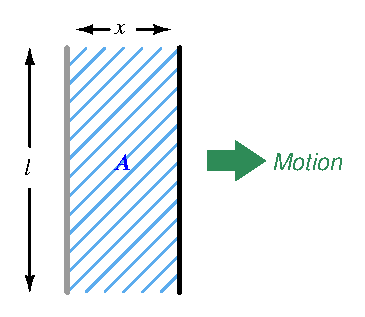
\includegraphics[width=15.5cm]{i00521x01.eps}$$

Hvis vi uttrykker $A$, $l$ og $x$ som vektorer, kan vi si at $\vec A = \vec l \times \vec x$. Hvis $l$ er konstant (slik den bør være!), kan ligningen $\vec A = \vec l \times \vec x$ deriveres slik:

$$d \vec A = \vec l \times d \vec x$$

Deretter setter vi inn $\vec l \times d \vec x$ for $d \vec A$ i integranden til Faradays ligning:

$$e = N {d \over dt} \int \vec B \cdot (\vec l \times d \vec x)$$

Vi vet selvfølgelig at hastighet $v$ er tidsderivert av strekning $x$:

$$v = {dx \over dt} \hbox{\hskip 30pt . . . eller . . . \hskip 30pt} dx = v \> dt$$

Nå setter vi inn $\vec v \> dt$ for $d \vec x$ i integranden til Faradays ligning:

$$e = N {d \over dt} \int \vec B \cdot (\vec l \times \vec v) \> dt$$

Derivasjon og integrasjon opphever da hverandre, siden begge er med hensyn på tid $t$:

$$e = N \vec B \cdot (\vec l \times \vec v)$$

Hvis det kun er én leder involvert, er $N = 1$, og vi kan skrive:

$$e = \vec B \cdot (\vec l \times \vec v)$$

Hvis vi vet at hastighetsvektoren ($\vec v$) står vinkelrett på lengdevektoren ($\vec l$), må kryssproduktet ($\vec A$) stå vinkelrett på begge. Hvis både $\vec v$ og $\vec l$ står vinkelrett på magnetfeltvektoren ($\vec B$), vil arealvektoren ($\vec A$) være parallell med feltvektoren, og skalarproduktet blir lik det vanlige skalaruttrykket:

$$e = Blv$$

%INDEX% Fysikk, elektrisitet: Faradays lov for elektromagnetisk induksjon

%(END_NOTES)

